\documentclass[10pt]{exam}

\usepackage{amssymb, amsmath, amsthm, mathrsfs, multicol, graphicx} 
\usepackage{tikz}

\def\d{\displaystyle}
\def\?{\reflectbox{?}}
\def\b#1{\mathbf{#1}}
\def\f#1{\mathfrak #1}
\def\c#1{\mathcal #1}
\def\s#1{\mathscr #1}
\def\r#1{\mathrm{#1}}
\def\N{\mathbb N}
\def\Z{\mathbb Z}
\def\Q{\mathbb Q}
\def\R{\mathbb R}
\def\C{\mathbb C}
\def\F{\mathbb F}
\def\A{\mathbb A}
\def\X{\mathbb X}
\def\E{\mathbb E}
\def\O{\mathbb O}
\def\pow{\mathscr P}
\def\inv{^{-1}}
\def\nrml{\triangleleft}
\def\st{:}
\def\~{\widetilde}
\def\rem{\mathcal R}
\def\iff{\leftrightarrow}
\def\Iff{\Leftrightarrow}
\def\and{\wedge}
\def\And{\bigwedge}
\def\AAnd{\d\bigwedge\mkern-18mu\bigwedge}
\def\Vee{\bigvee}
\def\VVee{\d\Vee\mkern-18mu\Vee}
\def\imp{\rightarrow}
\def\Imp{\Rightarrow}
\def\Fi{\Leftarrow}

\def\={\equiv}
\def\var{\mbox{var}}
\def\mod{\mbox{Mod}}
\def\Th{\mbox{Th}}
\def\sat{\mbox{Sat}}
\def\con{\mbox{Con}}
\def\bmodels{=\joinrel\mathrel|}
\def\iffmodels{\bmodels\models}
\def\dbland{\bigwedge \!\!\bigwedge}
\def\dom{\mbox{dom}}
\def\rng{\mbox{range}}
\DeclareMathOperator{\wgt}{wgt}

\def\circleA{(-.5,0) circle (1)}
\def\circleAlabel{(-1.5,.6) node[above]{$A$}}
\def\circleB{(.5,0) circle (1)}
\def\circleBlabel{(1.5,.6) node[above]{$B$}}
\def\circleC{(0,-1) circle (1)}
\def\circleClabel{(.5,-2) node[right]{$C$}}
\def\twosetbox{(-2,-1.5) rectangle (2,1.5)}
\def\threesetbox{(-2,-2.5) rectangle (2,1.5)}


\def\bar{\overline}

%\pointname{pts}
\pointsinmargin
\marginpointname{pts}
\marginbonuspointname{pts-bns}
\addpoints
\pagestyle{head}
\printanswers

\firstpageheader{Math 228}{\bf Homework 11}{Due: Wednesday, April 22}

\def\vertexsize{4pt}
\newcommand{\vtx}[2]{node[fill,circle,inner sep=0pt, minimum size=\vertexsize,label=#1:#2]{}}
\newcommand{\va}[1]{\vtx{above}{#1}}
\newcommand{\vb}[1]{\vtx{below}{#1}}
\newcommand{\vr}[1]{\vtx{right}{#1}}
\newcommand{\vl}[1]{\vtx{left}{#1}}
\renewcommand{\v}{\vtx{above}{}}

\begin{document}
\noindent \textbf{Instructions}: Same rules as usual - turn in your work on separate sheets of paper.  You must justify all your answers for full credit.

\begin{questions}

\question Edward A. Mouse has just finished his brand new house.  The floor plan is shown below:

\begin{center}
  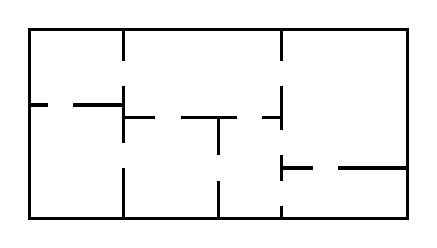
\begin{tikzpicture}[scale=.8]
    \draw[very thick] (-3,0) rectangle (3,3);
    \draw[very thick] (-3,1.8) --(-2.7,1.8) (-2.3,1.8) -- (-1.5, 1.8) (-1.5, 1.6) -- (-1,1.6) (-.6, 1.6) -- (.3,1.6) (.7,1.6) -- (1, 1.6) (1, .8) -- (1.5, .8) (1.9,.8) -- (3,.8); 
    \draw[very thick] (-1.5,0) -- (-1.5, .8) (-1.5, 1.2) -- (-1.5,2.1) (-1.5,2.5) -- (-1.5,3);
    \draw[very thick] (0,0) -- (0,.6) (0,1) -- (0,1.6);
    \draw[very thick] (1,0) -- (1,.2) (1,.6) -- (1,1) (1,1.4) -- (1,2.1) (1,2.5) -- (1,3);
  \end{tikzpicture}
\end{center}


\begin{parts}
 \part[3] Edward wants to give a tour of his new pad to a lady-mouse-friend.  Is it possible for them to walk through every doorway exactly once?  If so, in which rooms must they begin and end the tour? Explain.
 \begin{solution}
   Yes, he must start in the top right room and end in the bottom middle room, or vice versa.  This is because those are the two rooms with an odd number of doors.  
   
   In graph theory terms, if we place a vertex in each room and connect vertices if there is a door between their rooms, we are asking whether the graph has an Euler path.  The number of doors is the degree of the vertex, and a graph has an Euler path if and only if there are two or fewer vertices with odd degree.  In that case, the path must start at one of those odd degree vertices and end at the other.
 \end{solution}

\part[2] Is it possible to tour the house visiting each room exactly once (not necessarily using every doorway)?  Explain.

\begin{solution}
  Yes.  This does not correspond to an Euler path or circuit, since all we need to do is visit each vertex exactly once.  It is easy to do - for example, tour the house clockwise.
\end{solution}


\part[3] After a few mouse-years, Edward decides to remodel.  He would like to add some new doors between the rooms he has.  Of course, he cannot add any doors to the exterior of the house.  Is it possible for each room to have an odd number of doors? Explain.
\begin{solution}
  No it is not possible.  If each room had an odd number of doors, then the corresponding graph would have the property that the degree of every vertex would be odd.  There are 7 vertices, and if their degrees were all odd, then the sum of the degrees would be an odd number as well.  But the number of edges in a graph is always 1/2 the sum of the degrees, so the sum of the degrees must be even.
  
  In other words, if you add up the number of doors in all rooms, you need to get an even number, since the number of doorways is half this number - each doorway counts as a door in two rooms.
\end{solution}

\end{parts}

\question A group of 10 friends decides to head up to a cabin in the woods (where nothing could possibly go wrong).  Unfortunately, a number of these friends have dated each other in the past, and things are still a little awkward.  To get the cabin, they need to divide up into some number of cars, and no two people who dated should be in the same car.
\begin{parts}
  \part[3] What is the smallest number of cars you need if all the relationships were strictly heterosexual?  Represent an example of such a situation with a graph.  What kind of graph do you get?
  \begin{solution}
    2 cars are needed.  Since no boys dated boys and no girls dated girls, it is possible to separate the youths into cars by gender.  The corresponding graph (with vertices representing people and edges representing the fact that those people dated) would be bipartite - there are no edges between two boys and no edges between two girls.  
  \end{solution}
  
\part[3] Because a number of these friends dated there are also conflicts between friends of the same gender, listed below. Now what is the smallest number of conflict-free cars they could take to the cabin?

\begin{center}
\begin{tabular}{c*{10}{|c}}
Friend & A & B & C & D & E & F & G & H & I & J\\ \hline
Has a conflict with & B E J & A D G & H J & B F & A I  & D J & B & C I & E H J & A C F I 
\end{tabular}
\end{center}

\begin{solution}
Draw the graph where vertices represent the 10 people and edges representing conflicts.  Color the graph properly.  The chromatic number of the graph is 3 (and you know it can't be smaller because there is an odd cycle present in the graph).
\end{solution}

%\begin{tabular}{c|cl}
%\textbf{Friend:} & \textbf{Has a conflict with:} \\ \hline
%A & B E J\\
%B & A D G\\
%C & H J\\
%D & B F \\
%E & A I \\
%F & D J \\
%G & B\\
%H & C I\\
%I & E H J \\
%J & A C F I
%\end{tabular}


%  \part[3] What is the smallest number of cars you need if the relationships could be represented by the Petersen graph (above)?  Assume each person is represented by a vertex, and two people have dated if there is an edge between their vertices. Explain.
%  
%  \begin{solution}
%    3 cars are needed.  The Petersen graph is not bipartite, so 2 cars is not enough.  You can see this because there is an odd circuit.  It is not too difficult to assign vertices to cars (i.e., color the vertices) so that no two adjacent vertices are assigned the same car (color).    
%  \end{solution}

  \part[2] What do these questions have to do with coloring? 
  \begin{solution}
    We are really asking for the chromatic number of the graphs.  The smallest number of cars needed is the smallest number of colors needed for a proper vertex coloring.
  \end{solution}
\end{parts}

\question[6] We say that a graph has a {\em Hamilton path} if there is a path which visits each vertex exactly once (you do not need to use every edge in the path).  
\begin{parts}
  \part Suppose a graph has a Hamilton path.  What is the maximum number of vertices of degree one the graph can have?  Explain why your answer is correct.

  \begin{solution}
    Note that a vertex of degree one can only be the start or the end of a Hamilton path - if we go {\em to} a vertex of degree one, we are stuck there - we cannot use the same edge to leave the vertex, because doing so would bring us back to a vertex we have already visited.  If a graph has a Hamilton path, it might start at a vertex of degree one, end at a vertex of degree one, but there cannot be any other vertices of degree one.  Therefore a graph with a Hamilton path can have at most two vertices of degree one.
  \end{solution}

  \part Find a graph which does not have a Hamilton path even though no vertex has degree one.  Explain why your example works.
  
  \begin{solution}
    There are many such graphs.  Here are two examples:
    
    \begin{center}
      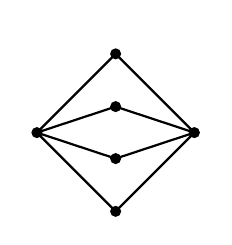
\begin{tikzpicture}
        \draw[thick] (-1,0) \v -- (0,1) \v -- (1, 0) \v -- (0, .33) \v -- (-1,0) -- (0,-.33) \v -- (1,0) -- (0,-1) \v -- (-1,0);
      \end{tikzpicture}
      \hspace{1in}
      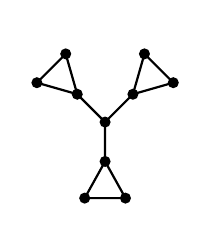
\begin{tikzpicture}
        \draw[thick] (270:.5) \v -- (255:1) \v -- (285:1) \v -- (270:.5) -- (0,0) \v -- (135:.5) \v -- (150:1) \v -- (120:1) \v -- (135:.5) (0,0) -- (45:.5) \v -- (60:1) \v -- (30:1) \v -- (45:.5);
      \end{tikzpicture}

    \end{center}

  \end{solution}

\end{parts}

\question Prove the chromatic number of any tree is two.
\begin{parts}
\part[2] Describe a procedure to color the tree below.

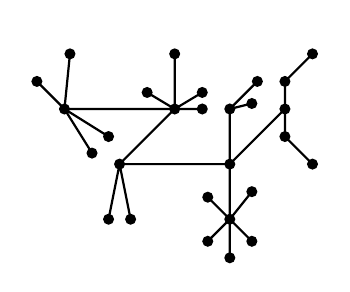
\begin{tikzpicture}[scale=.7]
\draw[thick] (-1,1) \v -- (-1.5,1.5) \v (-1,1) -- (-.9,2)\v (-1,1) -- (-.2,.5) \v (-1,1) -- (-.5,.2)\v;
\draw[thick] (-1,1) -- (1,1) \v -- (.5,1.3) \v (1,1) -- (1,2)\v (1,1) -- (1.5,1.3) \v (1,1) -- (1.5,1)\v;
\draw[thick] (1,1) -- (0,0) \v -- (-.2,-1) \v (0,0) -- (.2,-1) \v (0,0) -- (2,0) \v -- (2,1) \v -- (2.5,1.5) \v (2,1) -- (2.4,1.1) \v;
\draw[thick] (2,0) -- (2,-1) \v -- (2.4,-.5) \v (2,-1) -- (2.4, -1.4) \v (2,-1) -- (2,-1.7) \v (2,-1) -- (1.6,-1.4) \v (2,-1) -- (1.6,-.6) \v;
\draw[thick] (2,0) -- (3,1) \v -- (3,1.5) \v -- (3.5,2)\v (3,1) -- (3,.5) \v -- (3.5, 0) \v;
\end{tikzpicture}

\begin{solution}
Start with any vertex and color it blue.  Then look at all the neighbors of that vertex (i.e., those vertices that are connected to the vertex with and edge) and color all of these red.  Then look at all the neighbors of the red vertices and color them blue.  Then all the neighbors of the blue vertices (not yet colored) and color those red.  Keep going until all of the vertices are colored.
\end{solution}

%\part The chromatic number of $C_n$ is two when $n$ is even. What goes wrong when $n$ is odd?
\part[3] Prove that your procedure from part (a) always works for any tree.
\begin{solution}
You can always color the first vertex blue.  None of the neighbors of this vertex could be neighbors with each other, for this would create a cycle.  So all the neighbors can be colored red.  Now all the (uncolored) neighbors of the red vertices can be colored blue -- the only way this would fail is if one was already adjacent to the first vertex (but this is impossible because we already colored all its neighbors) or adjacent to each other, but this would create a cycle.  This continues at every step.
\end{solution}


\part[3] Now, prove using induction that every tree has chromatic number 2.
\begin{solution}
This proof is very similar to showing that every tree is a bipartite graph.\\
\begin{proof}
Let $P(n)$ be the statement ``A tree with $n$ vertices has a chromatic number of 2''\\
Base Case: Consider a tree with $3$ vertices. Since trees cannot have a cycle and two of the vertices are adjacent to the third vertex, we must have a coloring with 2 colors.\\
Inductive Case: Assume that $P(k)$ is true for some arbitrary $k<n$. Now, I need to show that $P(k+1)$ is true. So, I can assume that I have a tree with $k+1$ vertices and I must show that it has chromatic number 2. Now, if I remove one of leaf from the tree with $k+1$ vertices I will be removing exactly 1 edge and 1 vertex. Therefore I have a tree with $k$ vertices which I know by my inductive hypothesis must have a chromatic number of 2. Now, I can add that leaf back in, and since it's only attached to exactly one vertex which is colored one of the 2 colors, I can color the added vertex the opposite color and still have a chromatic number of 2. TBTPOMI $P(k+1)$ is true for all $n\geq 3$.
\end{proof} 
\end{solution}


\end{parts}

\bonusquestion[4] BONUS: King Arthur has hired a consultant, Sir Cumference, to plan a seating arrangement for Arthur and nine of his knights to sit around the round table. This would not be a difficult task, were it not for the jealousies and petty rivalries that exist among the knights. Arthur insists that Lancelot should sit on his right and that Kay should sit on his left; Bedivere refuses to sit next to anyone but Lionel and Tristan; Gawain won't sit next to Tristan, Lancelot, or Lionel; Gareth won't sit next to Galahad, Lancelot, or Kay; Perceval objects to sitting next to Galahad, Lancelot, or Lionel; Tristan refuses to sit next to Lancelot, Perceval or Kay; Galahad will sit next to anyone except Gawain and Kay; and Lionel will not sit next to Galahad. The other two knights are not particular about whom they sit next to. \\
Help Sir Cumference find a suitable seating arrangement and explain what this problem has to do with graphs.
\begin{solution}
Starting with Arthur and going clockwise the seating chart will be as follows: Arthur $\rightarrow$ Kay $\rightarrow$ Gawain $\rightarrow$ Perceval $\rightarrow$ Gareth $\rightarrow$ Lionel $\rightarrow$ Bedivere $\rightarrow$ Tristan $\rightarrow$ Galahad $\rightarrow$ Lancelot $\rightarrow$ Arthur.\\
Additionally, you could have switched Gawain and Perceval.
\end{solution}
\end{questions}




\end{document}


